\documentclass[12pt]{article}

\usepackage[left=0.9in,right=0.9in,top=0.8in,bottom=1.05in]{geometry}
\newcommand{\ligne}[1]{\rule[0.5ex]{\textwidth}{#1}\\}

\usepackage[]{graphicx}
\usepackage{amsmath}
%\usepackage{wrapfig}
%\usepackage{physics}

\begin{document}

\noindent
Sean Gravelle\\
Numerical PDEs Homework \#1\\

% \noindent \textbf{For all problems asking for a graph:} you do not need to write up the method you programmed. Including plots of your solution and convergence is sufficient for full credit. The ideal homework will have one, information-dense and properly labeled figure with a caption and a \textit{brief} discussion. \textbf{You must type up your HW.} I don't care if it's word or Tex as long as it's well organized, easy to follow, and submitted as a pdf. 

\vspace{0.3cm}

\subsection*{Problem 1: Solve Stokes}

My solution to the Stokes equations in 2 dimensions, with the given boundary conditions, is plotted below. I used $n=100=Nx=Ny$ gridpoints in both $x$ and $y$ directions.  Arrows indicate direction of the fluid's flow and color indicates the magnitude of the solution vector; that is, the speed of the fluid.

\begin{center}
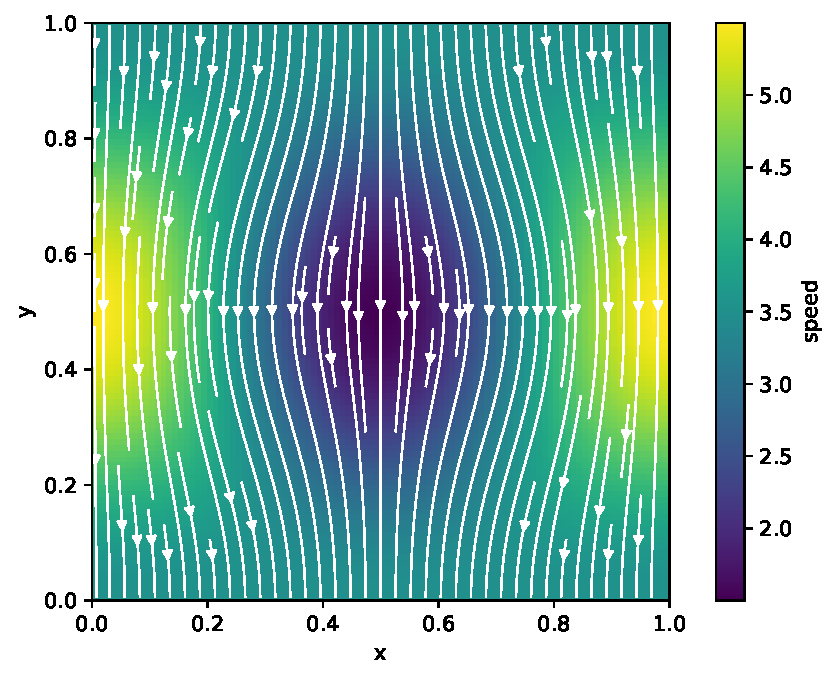
\includegraphics[width=\textwidth]{sol_plot.pdf}
\end{center}

\newpage
\subsection*{Problem 2: Error Analysis}

Plotting the relative error of numerical solutions on an $n\times n$ grid gives the following errors for $U$, $V$, and $P$. The slopes of each show that their errors decrease proportionally to $1/n^2$ (the second order baseline plotted as a black dashed line).

\begin{center}
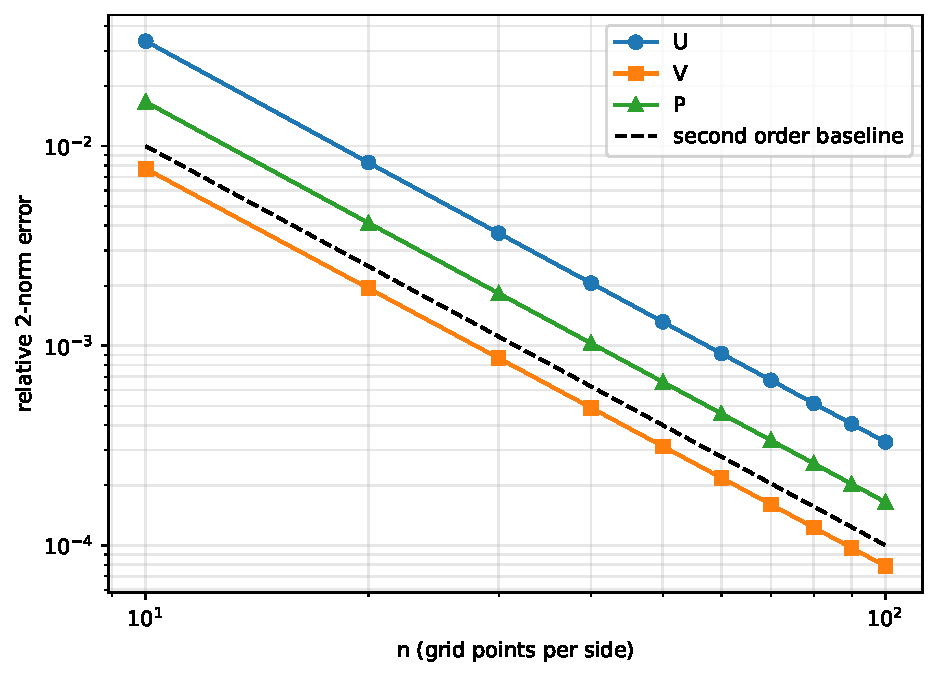
\includegraphics[width=\textwidth]{error_plot.pdf}
\end{center}

\newpage
\subsection*{Problem 3: Changing the boundary conditions}

I modified my code to solve the same PDE but with different boundary conditions on $U$:

\begin{itemize}
\item
On the left and right boundaries: Dirichlet condition $U=0$
\item
On the top and bottom boundaries: Neumann conditions $\partial U/\partial y =0$
\end{itemize}

I kept the same boundary conditions on $V$ and $P$ as in the original problem. Using the method of manufactured solutions, my analytic functions matching these boundary conditions are:

\begin{align*}
U_{an}(x,y) &= \cos(2\pi y)\sin(2\pi x) \\
V_{an}(x,y) &= -3.5-\cos(2\pi x)\sin(2\pi y) \\
P_{an}(x,y) &= \sin(2\pi y)\cos(2\pi x)
\end{align*}

My solution with these new boundary conditions is shown below.

\begin{center}
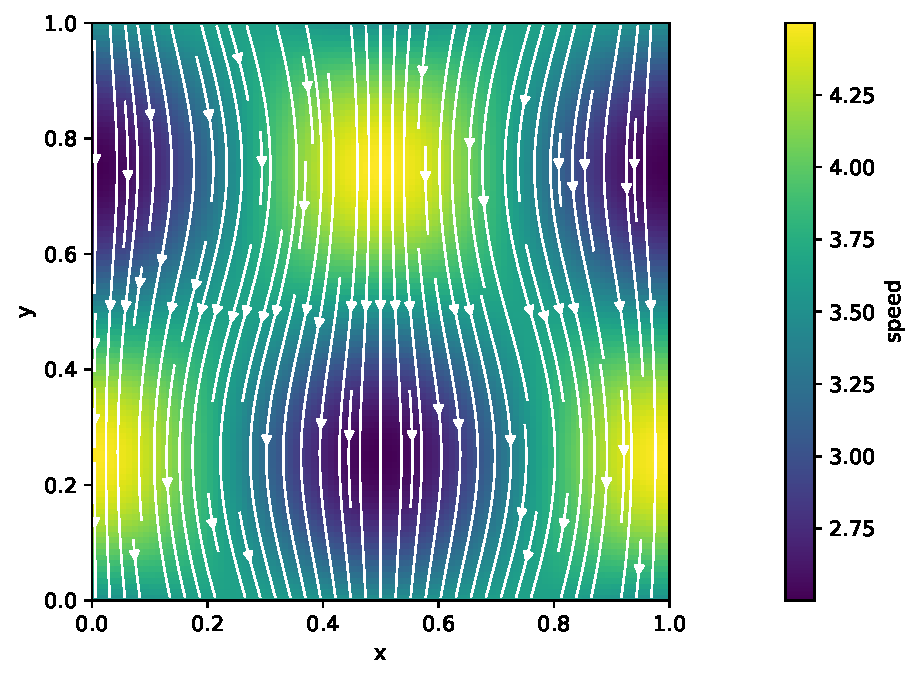
\includegraphics[width=\textwidth]{plot_new_bc.pdf}
\end{center}


\newpage

The plot below shows the error of my solution to the problem with modified boundary conditions. Error is measured in the 2-norm, as with the original problem. Second order accuracy is once again obtained.

\begin{center}
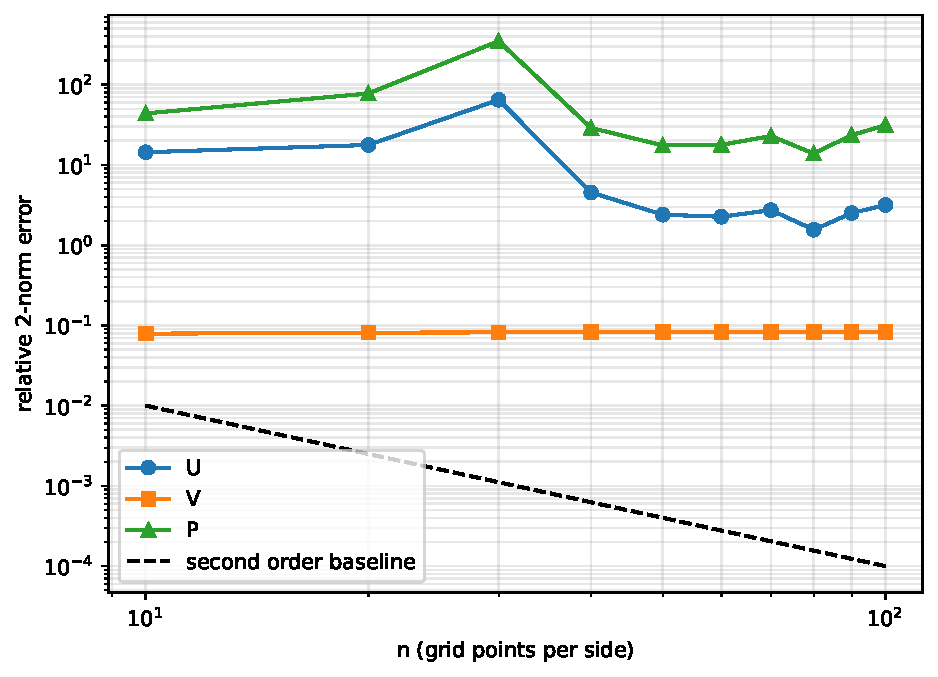
\includegraphics[width=\textwidth]{error_plot_new_bc.pdf}
\end{center}

\bigskip

\emph{AI disclosure statement:} All plots were made with LLM assistance. All mathematical work and all code to produce the numerical solutions and error calculations are my own, without LLM.


\end{document}